\chapter{Numbers and Storage Systems}
\label{chapter:numbers}

This chapter discusses how data are represented and stored in a computer.

In the context of computing, {\em boolean} refers to a condition that can
be either true or false and {\em binary} refers to the use of a base-2
numeric system to represent numbers.

RISC-V assembly language uses binary to represent all values, be they
boolean or numeric.  It is the context within which they are used that
determines whether they are boolean or numeric.

\ednote{Add some diagrams here showing bits, bytes and the MSB,
LSB,\ldots\ perhaps relocated from the RV32I chapter?}

\section{Boolean Functions}

Boolean functions apply on a per-bit basis.
When applied to multi-bit values, each bit position is operated upon
independent of the other bits.

RISC-V assembly language uses zero to represent {\em false} and one
to represent {\em true}.  In general, however, it is useful to relax
this and define zero {\bf and only zero} to be {\em false} and anything
that is not {\em false} is therefore {\em true}.%
\footnote{This is how {\em true} and {\em false} behave in C, C++, and
many other languages as well as the common assembly language idioms
discussed in this text.}

The reason for this relaxation is to describe the common case
where the CPU processes data, multiple \gls{bit}s at-a-time.

These
groups have names like \gls{byte} (8 bits), \gls{halfword} (16 bits)
and \gls{fullword} (32 bits).

\subsection{NOT}

The {\em NOT} operator applies to a single operand and represents the
opposite of the input.
\ednote{Need to define unary, binary and ternary operators without
confusing binary operators with binary numbers.}

If the input is 1 then the output is 0.  If the input is 0 then the
output is 1.  In other words, the output value is {\em not} that of the
input value.

Expressing the {\em not} function in the form of a truth table:

\begin{center}
\begin{tabular}{c|c}
A & $\overline{\mbox{A}}$\\
\hline
0 & 1 \\
1 & 0 \\
\end{tabular}
\end{center}

A truth table is drawn by indicating all of the possible input values on
the left of the vertical bar with each row displaying the output values
that correspond to the input for that row.  The column headings are used
to define the illustrated operation expressed using a mathematical
notation.  The {\em not} operation is indicated by the presence of
an {\em overline}.

In computer programming languages, things like an overline can not be
efficiently expressed using a standard keyboard.  Therefore it is common
to use a notation such as that used  by the C language when discussing
the {\em NOT} operator in symbolic form.  Specifically the tilde: `\verb@~@'.

It is also uncommon to for programming languages to express boolean operations
on single-bit input(s).  A more generalized operation is used that applies
to a set of bits all at once.  For example, performing a {\em not} operation
of eight bits at once can be illustrated as:


\begin{verbatim}
  ~ 1 1 1 1 0 1 0 1  <== A
  -----------------
    0 0 0 0 1 0 1 0  <== output
\end{verbatim}

In a line of code the above might read like this: \verb@output = ~A@

\subsection{AND}

The boolean {\em and} function has two or more inputs and the output is a
single bit.  The output is 1 if and only if all of the input values are 1.
Otherwise it is 0.

This function works like it does in spoken language.  For example
if A is 1 {\em and} B is 1 then the output is 1 (true).
Otherwise the output is 0 (false).

In mathematical notion, the {\em and} operator is expressed the same way
as is {\em multiplication}.  That is by a raised dot between, or by
juxtaposition of, two variable names.  It is also worth noting that,
in base-2, the {\em and} operation actually {\em is} multiplication!

\begin{center}
\begin{tabular}{cc|c}
A & B & AB \\
\hline
0 & 0 & 0 \\
0 & 1 & 0 \\
1 & 0 & 0 \\
1 & 1 & 1 \\
\end{tabular}
\end{center}

This text will use the operator used in the C language when discussing
the {\em and} operator in symbolic form.  Specifically the ampersand: `\verb@&@'.

An eight-bit example:

\begin{verbatim}
    1 1 1 1 0 1 0 1  <== A
  & 1 0 0 1 0 0 1 1  <== B
  -----------------
    1 0 0 1 0 0 0 1  <== output
\end{verbatim}

In a line of code the above might read like this: \verb@output = A & B@

\subsection{OR}

The boolean {\em or} function has two or more inputs and the output is a
single bit.  The output is 1 if at least one of the input values are 1.

This function works like it does in spoken language.  For example
if A is 1 {\em or} B is 1 then the output is 1 (true).
Otherwise the output is 0 (false).

In mathematical notion, the {\em or} operator is expressed using the plus
($+$).

\begin{center}
\begin{tabular}{cc|c}
A & B & A$+$B \\
\hline
0 & 0 & 0 \\
0 & 1 & 1 \\
1 & 0 & 1 \\
1 & 1 & 1 \\
\end{tabular}
\end{center}

This text will use the operator used in the C language when discussing
the {\em or}  operator in symbolic form.  Specifically the pipe: `\verb@|@'.

An eight-bit example:

\begin{verbatim}
    1 1 1 1 0 1 0 1  <== A
  | 1 0 0 1 0 0 1 1  <== B
  -----------------
    1 1 1 1 0 1 1 1  <== output
\end{verbatim}

In a line of code the above might read like this: \verb@output = A | B@

\subsection{XOR}

The boolean {\em exclusive or} function has two or more inputs and the
output is a single bit.  The output is 1 if only an odd number of inputs
are 1. Otherwise the output will be 0.

Note that when {\em xor} is used with two inputs, the output
is set to 1 (true) when the inputs have different values and 0
(false) when the inputs both have the same value.

In mathematical notion, the {\em xor} operator is expressed using the plus
in a circle ($\oplus$).

\begin{center}
\begin{tabular}{cc|c}
A & B & A$\oplus{}$B \\
\hline
0 & 0 & 0 \\
0 & 1 & 1 \\
1 & 0 & 1 \\
1 & 1 & 0 \\
\end{tabular}
\end{center}

This text will use the operator used in the C language when discussing
the {\em xor}  operator in symbolic form.  Specifically the carrot: `\verb@^@'.


An eight-bit example:

\begin{verbatim}
    1 1 1 1 0 1 0 1  <== A
  ^ 1 0 0 1 0 0 1 1  <== B
  -----------------
    0 1 1 0 0 1 1 0  <== output
\end{verbatim}

In a line of code the above might read like this: \verb@output = A ^ B@

\section{Integers and Counting}

A binary integer is constructed with only 1s and 0s in the same
manner as decimal numbers are constructed with values from 0 to 9.

Counting in binary (base-2) uses the same basic rules as decimal (base-10).
The difference is when we consider that there are ten decimal digits and
only two binary digits.  Therefore, in base-10, we must carry when adding one to
nine (because there is no digit representing a ten) and, in base-2, we must
carry when adding one to one (because there is no digit representing a two.)

\autoref{Figure:integers} shows an abridged table of the decimal, binary and
hexadecimal values ranging from $0_{10}$ to $128_{10}$.

\begin{figure}[t]
\begin{center}
\begin{tabular}{|c|c|c||c|c|c|c|c|c|c|c||c|c|}
\hline
\multicolumn{3}{|c||}{Decimal} & \multicolumn{8}{|c||}{Binary} & \multicolumn{2}{|c|}{Hex}\\
\hline
$10^2$	& $10^1$	& $10^0$	& $2^7$ & $2^6$ & $2^5$ & $2^4$ & $2^3$ & $2^2$ & $2^1$ & $2^0$		& $16^1$ & $16^0$	\\
\hline
100		&	10		& 1			& 128	& 64	& 32	& 16	& 8		& 4		& 2		& 1			& 16	& 1			\\
\hline \hline
0		&	0		&	0		& 0 & 0 & 0 & 0 & 0 & 0 & 0 & 0		& 0 & 0 \\
0		&	0		&	1		& 0 & 0 & 0 & 0 & 0 & 0 & 0 & 1		& 0 & 1 \\
0		&	0		&	2		& 0 & 0 & 0 & 0 & 0 & 0 & 1 & 0		& 0 & 2 \\
0		&	0		&	3		& 0 & 0 & 0 & 0 & 0 & 0 & 1 & 1		& 0 & 3 \\
0		&	0		&	4		& 0 & 0 & 0 & 0 & 0 & 1 & 0 & 0		& 0 & 4 \\
0		&	0		&	5		& 0 & 0 & 0 & 0 & 0 & 1 & 0 & 1		& 0 & 5 \\
0		&	0		&	6		& 0 & 0 & 0 & 0 & 0 & 1 & 1 & 0		& 0 & 6 \\
0		&	0		&	7		& 0 & 0 & 0 & 0 & 0 & 1 & 1 & 1		& 0 & 7 \\
0		&	0		&	8		& 0 & 0 & 0 & 0 & 1 & 0 & 0 & 0		& 0 & 8 \\
0		&	0		&	9		& 0 & 0 & 0 & 0 & 1 & 0 & 0 & 1		& 0 & 9 \\
0		&	1		&	0		& 0 & 0 & 0 & 0 & 1 & 0 & 1 & 0		& 0 & a \\
0		&	1		&	1		& 0 & 0 & 0 & 0 & 1 & 0 & 1 & 1		& 0 & b \\
0		&	1		&	2		& 0 & 0 & 0 & 0 & 1 & 1 & 0 & 0		& 0 & c \\
0		&	1		&	3		& 0 & 0 & 0 & 0 & 1 & 1 & 0 & 1		& 0 & d \\
0		&	1		&	4		& 0 & 0 & 0 & 0 & 1 & 1 & 1 & 0		& 0 & e \\
0		&	1		&	5		& 0 & 0 & 0 & 0 & 1 & 1 & 1 & 1		& 0 & f \\
0		&	1		&	6		& 0 & 0 & 0 & 1 & 0 & 0 & 0 & 0		& 1 & 0 \\
0		&	1		&	7		& 0 & 0 & 0 & 1 & 0 & 0 & 0 & 1		& 1 & 1 \\
\hline
\multicolumn{3}{|c||}{\ldots} & \multicolumn{8}{|c||}{\ldots} & \multicolumn{2}{|c|}{\ldots}\\
\hline
1       &   2       &   5		& 0 & 1 & 1 & 1 & 1 & 1 & 0 & 1		& 7 & d \\
1       &   2       &   6		& 0 & 1 & 1 & 1 & 1 & 1 & 1 & 0		& 7 & e \\
1       &   2       &   7		& 0 & 1 & 1 & 1 & 1 & 1 & 1 & 1		& 7 & f \\
1       &   2       &   8		& 1 & 0 & 0 & 0 & 0 & 0 & 0 & 0		& 8 & 0 \\
\hline
\end{tabular}
\end{center}
\captionof{figure}{Counting in decimal, binary and hexadecimal.}
\label{Figure:integers}
\end{figure}

One way to look at this table is on a per-row basis where each
\gls{place-value}
is represented by the base raised to the power of the \gls{place-value}
position (shown in the column headings.)
%This is useful when converting arbitrary numeric values between bases.
For example to interpret the decimal value on the fourth row:

\begin{equation}
0 \times 10^2 + 0 \times 10^1 + 3 \times 10^0 = 3_{10}
\end{equation}

Interpreting the binary value on the fourth row by converting it to decimal:

\begin{equation}
0 \times 2^7 + 0 \times 2^6 +0 \times 2^5 +0 \times 2^4 +0 \times 2^3 +0 \times 2^2 + 1 \times 2^1 + 1 \times 2^0 = 3_{10}
\end{equation}

Interpreting the hexadecimal value on the fourth row by converting it to decimal:

\begin{equation}
0 \times 16^1 + 3 \times 16^0 = 3_{10}
\end{equation}

\index{Most significant bit}\index{MSB|see {Most significant bit}}%
\index{Least significant bit}\index{LSB|see {Least significant bit}}%
We refer to the place values with the largest exponent (the one furthest to the
left for any given base) as the most significant digit and the place value
with the lowest exponent as the least significant digit.  For binary
numbers these are the \acrfull{msb} and \acrfull{lsb} respectively.%
\footnote{Changing the value of the MSB will have a more {\em significant}
impact on the numeric value than changing the value of the LSB.}

Another way to look at this table is on a per-column basis.  When
tasked with drawing such a table by hand, it might be useful
to observe that, just as in decimal, the right-most column will
cycle through all of the values represented in the chosen base
then cycle back to zero and repeat.  (For example, in binary this
pattern is 0-1-0-1-0-1-0-\ldots) The next column in each base
will cycle in the same manner except each of the values is repeated
as many times as is represented by the place value (in the case of
decimal, $10^1$ times, binary $2^1$ times, hex $16^1$ times.  Again,
the binary numbers for this pattern are 0-0-1-1-0-0-1-1-\ldots)
This continues for as many columns as are needed to represent the
magnitude of the desired number.

Another item worth noting is that any even binary number will always
have a 0 LSB and odd numbers will always have a 1 LSB.

As is customary in decimal, leading zeros are sometimes not shown
for readability.

The relationship between binary and hex values is also worth taking
note.  Because $2^4 = 16$, there is a clean and simple grouping
of 4 \gls{bit}s to 1 \gls{hit} (aka \gls{nybble}).
There is no such relationship between binary and decimal.

Writing and reading numbers in binary that are longer than 8 bits
is cumbersome and prone to error.  The simple conversion between
binary and hex makes hex a convenient shorthand for expressing
binary values in many situations.

For example, consider the following value expressed in binary,
hexadecimal and decimal (spaced to show the relationship
between binary and hex):

\begin{verbatim}
Binary value:       0010 0111 1011 1010 1100 1100 1111 0101
Hex Value:             2    7    B    A    C    C    F    5
Decimal Value:                                    666553589
\end{verbatim}

Empirically we can see that grouping the bits into sets of four
allows an easy conversion to hex and expressing it as such is
$\frac{1}{4}$ as long as in binary while at the same time
allowing for easy conversion back to binary.

The decimal value in this example does not easily convey a sense
of the binary value.

\begin{tcolorbox}
In programming languages like the C, its derivatives and RISC-V
assembly, numeric values are interpreted as decimal {\bfseries unless}
they start with a zero (0).
Numbers that start with 0 are interpreted as octal (base-8),
numbers starting with 0x are interpreted as hexadecimal and
numbers that start with 0b are interpreted as binary.
\end{tcolorbox}

%%%%%%%%%%%%%%%%%%%%%%%%%%%%%%%%%%%%%%%%%%%%%%%%%%%%%%%%%%%%%%%%%%%%%%%%%
%%%%%%%%%%%%%%%%%%%%%%%%%%%%%%%%%%%%%%%%%%%%%%%%%%%%%%%%%%%%%%%%%%%%%%%%%%
\subsection{Converting Between Bases}

%%%%%%%%%%%%%%%%%%%%%%%%%%%%%%%%%%%%%%%%%%%%%%%%%%%%%%%%%%%%%%%%%%%%%%%%%%
\subsubsection{From Binary to Decimal}
\label{section:bindec}

It is occasionally necessary to convert between decimal,
binary and/or hex.

To convert from binary to decimal, put the decimal value of the \gls{place-value}s
{\ldots8, 4, 2, 1} over the binary digits like this:

\begin{verbatim}
Base-2 place values: 128 64 32 16  8  4  2  1
Binary:                0  0  0  1  1  0  1  1
Decimal:                       16 +8    +2 +1 = 27
\end{verbatim}

Now sum the place-values that are expressed in decimal for each
bit with the value of 1: $16+8+2+1$.  The integer binary value
$00011011_2$ represents the decimal value $27_{10}$.

%%%%%%%%%%%%%%%%%%%%%%%%%%%%%%%%%%%%%%%%%%%%%%%%%%%%%%%%%%%%%%%%%%%%%%%%%%
\subsubsection{From Binary to Hexadecimal}
\label{section:binhex}

Conversion from binary to hex involves grouping the bits into
sets of four and then performing the same summing process as
shown above.  If there is not a multiple of four bits then
extend the binary to the left with zeros to make it so.

Grouping the bits into sets of four and summing:

\begin{verbatim}
Base-2 place values:   8 4 2 1     8 4 2 1     8 4 2 1     8 4 2 1
Binary:                0 1 1 0     1 1 0 1     1 0 1 0     1 1 1 0
Decimal:                 4+2  =6   8+4+  1=13  8+  2  =10  8+4+2  =14
\end{verbatim}

After the summing, convert each decimal value to hex.  The decimal
values from 0--9 are the same values in hex.  Because we don't have any
more numerals to represent the values from 10-15, we use the first 6
letters (See the right-most column of \autoref{Figure:integers}.)
Fortunately there are only six hex mappings involving letters.  Thus
it is reasonable to memorize them.

Continuing this example:

\begin{verbatim}
Decimal:               6           13          10          14
Hex:                   6           D           A           E
\end{verbatim}



%%%%%%%%%%%%%%%%%%%%%%%%%%%%%%%%%%%%%%%%%%%%%%%%%%%%%%%%%%%%%%%%%%%%%%%%%%
\subsubsection{From Hexadecimal to Binary}

The four-bit mapping between binary and hex makes this
task as straight forward as using a look-up table to
translate each \gls{hit} (Hex digIT) it to its unique
four-bit pattern.

Perform this task either by memorizing each of the 16 patterns
or by converting each hit to decimal first and then converting
each four-bit binary value to decimal using the place-value summing
method discussed in \autoref{section:bindec}.

For example:

\begin{verbatim}
Hex:                     7          C
Decimal Sum:       4+2+1=7  8+4    =12
Binary:          0 1 1 1    1 1 0 0
\end{verbatim}


%%%%%%%%%%%%%%%%%%%%%%%%%%%%%%%%%%%%%%%%%%%%%%%%%%%%%%%%%%%%%%%%%%%%%%%%%%
\subsubsection{From Decimal to Binary}

To convert arbitrary decimal numbers to binary, extend the list
of binary place values until it exceeds the value of the decimal
number being converted.  Then make successive subtractions of each
of the place values that would yield a non-negative result.

For example, to convert $1234_{10}$ to binary:


\begin{verbatim}
Base-2 place values: 2048-1024-512-256-128-64-32-16-8-4-2-1

   0          2048      (too big)
   1   1234 - 1024 = 210
   0          512       (too big)
   0          256       (too big)
   1    210 - 128  = 82
   1     82 - 64   = 18
   0          32        (too big)
   1     18 - 16   = 2
   0          8         (too big)
   0          4         (too big)
   1      2 - 2    = 0
   0          1         (too big)
\end{verbatim}

The answer using this notation is listed vertically
in the left column with the \acrshort{msb} on the top and
the \acrshort{lsb} on the bottom line: $010011010010_2$.


%%%%%%%%%%%%%%%%%%%%%%%%%%%%%%%%%%%%%%%%%%%%%%%%%%%%%%%%%%%%%%%%%%%%%%%%%%
\subsubsection{From Decimal to Hex}

Conversion from decimal to hex can be done by using the place
values for base-16 and the same math as from decimal to binary
or by first converting the decimal value to binary and then
from binary to hex by using the methods discussed above.

Because binary and hex are so closely related, performing
a conversion by way of binary is straight forward.


%%%%%%%%%%%%%%%%%%%%%%%%%%%%%%%%%%%%%%%%%%%%%%%%%%%%%%%%%%%%%%%%%%%%%%%%%
%%%%%%%%%%%%%%%%%%%%%%%%%%%%%%%%%%%%%%%%%%%%%%%%%%%%%%%%%%%%%%%%%%%%%%%%%%
\subsection{Addition of Binary Numbers}

The addition of binary numbers can be performed long-hand the
same way decimal addition is taught in grade school.  In fact binary
addition is easier since it only involves adding 0 or 1.

The first thing to note that in any number base $0+0=0$, $0+1=1$, and
$1+0=1$.  Since there is no ``two'' in binary (just like there is
no ``ten'' decimal) adding $1+1$ results in a zero with a carry as
in: $1+1=10_2$ and in: $1+1+1=11_2$.  Using these five sums, any two
binary integers can be added.

\index{Full Adder}%
This truth table shows what is called a {\em Full Addr}.
A full addr is a function that can add three input bits
(the two addends and a carry value from a ``prior column'')
and produce the sum and carry output values.\footnote{
Note that the sum could be expressed in Boolean Algebra as:
$sum = ci \oplus{} a \oplus{} b$}

\begin{center}
\begin{tabular}{|ccc|cc|}
\hline
%\multicolumn{3}{c}{input} & \multicolumn{2}{c}{output}\\
$ci$ & $a$ & $b$ & $co$ & $sum$\\
\hline
 0 & 0 & 0 &   0 & 0 \\
 0 & 0 & 1 &   0 & 1 \\
 0 & 1 & 0 &   0 & 1 \\
 0 & 1 & 1 &   1 & 0 \\
 1 & 0 & 0 &   0 & 1 \\
 1 & 0 & 1 &   1 & 0 \\
 1 & 1 & 0 &   1 & 0 \\
 1 & 1 & 1 &   1 & 1 \\
\hline
\end{tabular}
\end{center}

Adding two unsigned binary numbers using 16 full adders:

\begin{verbatim}
        111111  1111  <== carries
     0110101111001111 <== addend
   + 0000011101100011 <== addend
   ------------------
     0111001100110010 <== sum
\end{verbatim}

Note that the carry ``into'' the LSB is zero.



%%%%%%%%%%%%%%%%%%%%%%%%%%%%%%%%%%%%%%%%%%%%%%%%%%%%%%%%%%%%%%%%%%%%%%%%%%
%%%%%%%%%%%%%%%%%%%%%%%%%%%%%%%%%%%%%%%%%%%%%%%%%%%%%%%%%%%%%%%%%%%%%%%%%
\subsection{Signed Numbers}

There are multiple methods used to represent signed binary integers.
The method used by most modern computers is called {\em two's complement}.

A two's complement number is encoded in such a manner as to simplify
the hardware used to add, subtract and compare integers.

A simple method of thinking about two's complement numbers is to
negate the place value of the \acrshort{msb}.  For example, the
number one is represented the same as discussed before:

\begin{verbatim}
Base-2 place values:  -128 64 32 16  8  4  2  1
Binary:                  0  0  0  0  0  0  0  1
\end{verbatim}

The \acrshort{msb} of any negative number in this format will always
be 1.  For example the value $-1_{10}$ is:

\begin{verbatim}
Base-2 place values:  -128 64 32 16  8  4  2  1
Binary:                  1  1  1  1  1  1  1  1
\end{verbatim}

\ldots because: $-128+64+32+16+8+4+2+1=-1$.

This format has the virtue of allowing the same addition logic discussed above to be
used to calculate the sums of signed numbers as unsigned numbers.

Calculating the signed addition: $4+5 = 9$

\begin{verbatim}
       1    <== carries
     000100 <== 4 = 0 + 0 + 0 + 4 + 0 + 0
    +000101 <== 5 = 0 + 0 + 0 + 4 + 0 + 1
    -------
     001001 <== 9 = 0 + 0 + 8 + 0 + 0 + 1
\end{verbatim}

Calculating the signed addition: $-4+ -5 = -9$

\begin{verbatim}
    1 11     <== carries
      111100 <== -4 = -32 + 16 + 8 + 4 + 0 + 0
     +111011 <== -5 = -32 + 16 + 8 + 0 + 2 + 1
   ---------
    1 110111 <== -9 (with a truncation) = -32 + 16 + 4 + 2 + 1 = -9
\end{verbatim}


Calculating the signed addition: $-1+1=0$

\begin{verbatim}
   -128 64 32 16  8  4  2  1 <== place value
   1  1  1  1  1  1  1  1    <== carries
      1  1  1  1  1  1  1  1 <== addend (-1)
    + 0  0  0  0  0  0  0  1 <== addend (1)
      ----------------------
   1  0  0  0  0  0  0  0  0 <== sum (0 with a truncation)
\end{verbatim}

{\em In order for this to work, the carry out of the sum of the MSBs {\bfseries must} be discarded.}

%%%%%%%%%%%%%%%%%%%%%%%%%%%%%%%%%%%%%%%%%%%%%%%%%%%%%%%%%%%%%%%%%%%%%%%%%%
\subsubsection{Converting between Positive and Negative}

Changing the sign on two's complement numbers can be described as
inverting all of the bits (which is also known as the {\em one's complement})
and then add one.

For example, negating the number four:

\begin{minipage}{\textwidth}
\begin{verbatim}
   -128 64 32 16  8  4  2  1
      0  0  0  0  0  1  0  0 <== 4

                     1  1    <== carries
      1  1  1  1  1  0  1  1 <== one's complement of 4
    + 0  0  0  0  0  0  0  1 <== plus 1
      ----------------------
      1  1  1  1  1  1  0  0 <== -4
\end{verbatim}
\end{minipage}

This can be verified by adding 5 to the result and observe that
the sum is 1:

\begin{verbatim}
   -128 64 32 16  8  4  2  1
  1   1  1  1  1  1          <== carries
      1  1  1  1  1  1  0  0 <== -4
    + 0  0  0  0  0  1  0  1 <== 5
      ----------------------
  1   0  0  0  0  0  0  0  1 <== 1 (with a truncation)
\end{verbatim}

Note that the changing of the sign using this method is symmetric
in that it is identical when converting from negative to positive
and when converting from positive to negative: {\em flip the bits and
add 1.}

For example, changing the value -4 to 4 to illustrate the
reverse of the conversion above:

\begin{verbatim}
   -128 64 32 16  8  4  2  1
      1  1  1  1  1  1  0  0 <== -4

                     1  1    <== carries
      0  0  0  0  0  0  1  1 <== one's complement of -4
    + 0  0  0  0  0  0  0  1 <== plus 1
      ----------------------
      0  0  0  0  0  1  0  0 <== 4
\end{verbatim}

%%%%%%%%%%%%%%%%%%%%%%%%%%%%%%%%%%%%%%%%%%%%%%%%%%%%%%%%%%%%%%%%%%%%%%%%%
%%%%%%%%%%%%%%%%%%%%%%%%%%%%%%%%%%%%%%%%%%%%%%%%%%%%%%%%%%%%%%%%%%%%%%%%%%
\subsection{Subtraction of Binary Numbers}


Subtraction%
\ednote{This section needs more examples of subtracting
signed an unsigned numbers and a discussion on how
signedness is not relevant until the results are interpreted.
For example adding $-4+ -8=-12$ using two 8-bit numbers
is the same as adding $252+248=500$ and truncating the result
to 244.}
of binary numbers is performed by first negating
the subtrahend and then adding the two numbers.  Due to the
nature of two's complement numbers this method will work for both
signed and unsigned numbers!

Observation: Since we always have a carry-in of zero into the LSB when
adding, we can take advantage of that fact by (ab)using that carry input
to perform that adding the extra 1 to the subtrahend as part of
changing its sign in the examples below.

An example showing the subtraction of two {\em signed} binary numbers: $-4-8 = -12$

\begin{verbatim}
   -128 64 32 16  8  4  2  1
      1  1  1  1  1  1  0  0 <== -4  (minuend)
    - 0  0  0  0  1  0  0  0 <== 8   (subtrahend)
    ------------------------


  1   1  1  1  1  1  1  1  1 <== carries
      1  1  1  1  1  1  0  0 <== -4
    + 1  1  1  1  0  1  1  1 <== one's complement of 8
    ------------------------
  1   1  1  1  1  0  1  0  0 <== -12
\end{verbatim}


%An example showing the subtraction of two {\em unsigned} binary numbers: $252+248=500$
%
%\begin{verbatim}
%    128 64 32 16  8  4  2  1
%
%  1   1  1  1  1             <== carries
%      1  1  1  1  1  1  0  0 <== 252
%    + 1  1  1  1  1  0  0  0 <== 248
%      ----------------------
%  1   1  1  1  1  0  1  0  0 < == 500 (if we do NOT truncate the MSB)
%\end{verbatim}
%
%An example showing the subtraction of two {\em unsigned} binary numbers: $252+248=500$



%%%%%%%%%%%%%%%%%%%%%%%%%%%%%%%%%%%%%%%%%%%%%%%%%%%%%%%%%%%%%%%%%%%%%%%%%
%%%%%%%%%%%%%%%%%%%%%%%%%%%%%%%%%%%%%%%%%%%%%%%%%%%%%%%%%%%%%%%%%%%%%%%%%
\subsection{Truncation}
\index{truncation}
\index{overflow}
\index{carry}

Discarding the carry bit that can be generated from the MSB is called {\em truncation}.

So far we have been ignoring the carries that can come from the MSBs when adding and subtracting.
We have also been ignoring the potential impact of a carry causing a signed number to change
its sign in an unexpected way.

In the examples above, truncating the results either had 1) no impact on the calculated sums
or 2) was absolutely necessary to correct the sum in cases such as: $-4 + 5$.

For example, note what happens when we try to subtract 1 from the most
negative value that we can represent in a 4 bit two's complement number:

\begin{verbatim}
     -8  4  2  1
      1  0  0  0 <== -8  (minuend)
    - 0  0  0  1 <==  1  (subtrahend)
    ------------


   1           1 <== carries
      1  0  0  0 <== -8
    + 1  1  1  0 <== one's complement of 1
      ----------
   1  0  1  1  1 <== this SHOULD be -9 but with truncation it is 7
\end{verbatim}

The problem with this example is that we can not represent $-9_{10}$ using a 4-bit
two's complement number.

Granted, if we would have used 5 bit numbers, then the ``answer'' would have fit OK.
But the same problem would return when trying to calculate $-16 - 1$.
So simply ``making more room'' does not solve this problem.

%However, as calculating $-1+1=0$ has demonmstrated above, it was necessary for that
%case to discard the carry out of the MSB to get the correct result.

%In the case of calculating $-1+1=0$ the addends and result all fit into same-sized
%(8-bit) values. When calculating $-8-1=-9$ the addends each can fit into 4-bit
%two's complement numbers but the result would require a 5-bit number.

This is not just a problem when subtracting, nor is it just a problem with
signed numbers.

The same situation can happen {\em unsigned} numbers.
For example:

\begin{verbatim}
      8  4  2  1
  1   1  1  0  0 <== carries
      1  1  1  0 <== 14  (addend)
    + 0  0  1  1 <==  3  (addend)
    ------------
  1   0  0  0  1 <== this SHOULD be 17 but with truncation it is 1
\end{verbatim}


How to handle such a truncation depends on whether the {\em original} values
being added are signed or unsigned.

The RV ISA refers to the discarding the carry out of the MSB after an
add (or subtract) of two {\em unsigned} numbers as an {\em unsigned overflow}%
\footnote{Most microprocessors refer to {\em unsigned overflow} simply as a
{\em carry} condition.}
and the situation where carries create an incorrect sign in the
result of adding (or subtracting) two {\em signed} numbers as a
{\em signed overflow}.~\cite[p.~13]{rvismv1v22:2017}

\subsubsection{Unsigned Overflow}
\index{overflow!unsigned}

When adding {\em unsigned} numbers, an overflow only occurs when there
is a carry out of the MSB resulting in a sum that is truncated to fit
into the number of bits allocated to contain the result.

\autoref{sum:240+17} illustrates an unsigned overflow during addition:

\begin{figure}[H]
\centering
\begin{BVerbatim}
   1  1 1 1 0 0 0 0 0 <== carries
      1 1 1 1 0 0 0 0 <== 240
 +    0 0 0 1 0 0 0 1 <== 17
---------------------
   1  0 0 0 0 0 0 0 1 <== sum = 1
\end{BVerbatim}
%{\captionof{figure}{$240+16=0$ (overflow)}\label{sum:240+17}}
\caption{$240+17=1$ (overflow)}
\label{sum:240+17}
\end{figure}

Some times an overflow like this is referred to as a {\em wrap around}
because of the way that successive additions will result in a value that
increases until it {\em wraps} back {\em around} to zero and then
returns to increasing in value until it, again, wraps around again.

\begin{tcolorbox}
When adding, {\em unsigned overflow} occurs when ever there is a carry
{\em out of} the most significant bit.
\end{tcolorbox}

When subtracting {\em unsigned} numbers, an overflow only occurs when the
subtrahend is greater than the minuend (because in those cases the
different would have to be negative and there are no negative values
that can be represented with an unsigned binary number.)

\autoref{sum:3-4} illustrates an unsigned overflow during subtraction:

\begin{figure}[H]
\centering
\begin{BVerbatim}
     0 0 0 0 0 0 1 1 <== 3 (minuend)
   - 0 0 0 0 0 1 0 0 <== 4 (subtrahend)
   -----------------


  0  0 0 0 0 0 1 1 1 <== carries
     0 0 0 0 0 0 1 1 <== 3
   + 1 1 1 1 1 0 1 1 <== one's complement of 4
   -----------------
     1 1 1 1 1 1 1 1 <== 255 (overflow)
\end{BVerbatim}
\caption{$3-4=255$ (overflow)}
\label{sum:3-4}
\end{figure}

\begin{tcolorbox}
When subtracting, {\em unsigned overflow} occurs when ever there is {\em not} a carry
{\em out of} the most significant bit (IFF the carry-in on the LSB is used to add the
extra 1 to the subtrahend when changing its sign.)
\end{tcolorbox}


%%%%%%%%%%%%%%%%%%%%%%%%%%%%%%%%%%%%%%%%%%%%%%%%%%%%%%%%%%%%%%%%%%%%%%%%%
\subsubsection{Signed Overflow}
\index{overflow!signed}

When adding {\em signed} numbers, an overflow only occurs when the two
addends are positive and sum is negative or the addends are both negative
and the sum is positive.

When subtracting {\em signed} numbers, an overflow only occurs when the
minuend is positive and the subtrahend is negative and difference is negative
or when the minuend is negative and the subtrahend is positive and the
difference is positive.%
\footnote{I had to look it up to remember which were which
too\ldots\ it is: minuend - subtrahend = difference.\cite{subtrahend}}

Consider the results of the addition of two {\em signed} numbers
while looking more closely at the carry values.

\begin{figure}[H]
\centering
\begin{BVerbatim}
   0 1 0 0 0 0 0 0 0 <== carries
     0 1 0 0 0 0 0 0 <== 64
 +   0 1 0 0 0 0 0 0 <== 64
---------------------
     1 0 0 0 0 0 0 0 <== sum = -128
\end{BVerbatim}
\caption{$64+64 = -128$ (overflow)}
\label{sum:64+64}
\end{figure}



\autoref{sum:64+64} is an example of {\em signed overflow}.  As shown, the problem is
that the sum of two positive numbers has resulted in an obviously incorrect
negative result due to a carry flowing into the sign-bit in the MSB.

Granted, if the same values were added using values larger than 8-bits
then the sum would have been correct.  However, these examples assume that
all the operations are performed on (and results stored into) 8-bit values.
Given any finite-number of bits, there are values that could be added such that
an overflow occurs.

\index{truncation}
\autoref{sum:-128+-128} shows another overflow situation that is caused
by the fact that there is nowhere for the carry out of the sign-bit to go.
We say that this result has been {\em truncated}.

\begin{figure}[H]
\centering
\begin{BVerbatim}
   1 0 0 0 0 0 0 0 0 <== carries
     1 0 0 0 0 0 0 0 <== -128
 +   1 0 0 0 0 0 0 0 <== -128
---------------------
     0 0 0 0 0 0 0 0 <== sum = 0
\end{BVerbatim}
\caption{$-128+-128 = 0$ (overflow)}
\label{sum:-128+-128}
\end{figure}

Truncation is not necessarily a problem.  Consider the truncations in
figures \ref{sum:-3+-5} and \ref{sum:-2+10}.
\autoref{sum:-2+10} demonstrates the importance of discarding
the carry from the sum of the MSBs of signed numbers when addends
do not have the same sign.

\begin{figure}[H]
\centering
\begin{BVerbatim}
   1 1 1 1 1 1 1 1 0 <== carries
     1 1 1 1 1 1 0 1 <== -3
 +   1 1 1 1 1 0 1 1 <== -5
---------------------
     1 1 1 1 1 0 0 0  <== sum = -8
\end{BVerbatim}
\captionof{figure}{$-3+-5 = -8$}
\label{sum:-3+-5}
\end{figure}

\begin{figure}[H]
\centering
\begin{BVerbatim}
   1 1 1 1 1 1 1 0 0 <== carries
     1 1 1 1 1 1 1 0 <== -2
 +   0 0 0 0 1 0 1 0 <== 10
---------------------
     0 0 0 0 1 0 0 0 <== sum = 8
\end{BVerbatim}
\captionof{figure}{$-2+10 = 8$}
\label{sum:-2+10}
\end{figure}

Just like an unsigned number can wrap around as a result of
successive additions, a signed number can so the same thing.  The
only difference is that signed numbers won't wrap from the maximum
value back to zero, instead it will wrap from the most positive to
the most negative value as shown in \autoref{sum:127+1}.

\begin{figure}[H]
\centering
\begin{BVerbatim}
   0 1 1 1 1 1 1 1 0 <== carries
     0 1 1 1 1 1 1 1 <== 127
 +   0 0 0 0 0 0 0 1 <== 1
---------------------
     1 0 0 0 0 0 0 0 <== sum = -128
\end{BVerbatim}
\captionof{figure}{$127+1 = -128$}
\label{sum:127+1}
\end{figure}

\begin{tcolorbox}
Formally, a {\em signed overflow} occurs when ever the carry
{\em into} the most significant bit is not the same as the
carry {\em out of} the most significant bit.
\end{tcolorbox}

\section{Sign and Zero Extension}

\index{sign extension}
\label{SignExtension}
Due to the nature of the two's complement encoding scheme, the following
numbers all represent the same value:
\begin{verbatim}
                                   1111 <== -1
                               11111111 <== -1
                   11111111111111111111 <== -1
           1111111111111111111111111111 <== -1
\end{verbatim}
As do these:
\begin{verbatim}
                                  01100 <== 12
                             0000001100 <== 12
    00000000000000000000000000000001100 <== 12
\end{verbatim}

The lengthening of these numbers by replicating the digits on the left
is what is called {\em sign extension}.

\begin{tcolorbox}
Any signed number can have any quantity of additional MSBs added to it,
provided that they repeat the value of the sign bit.
\end{tcolorbox}

\autoref{Figure:SignExtendNegative} illustrates extending the negative sign
bit to the left by replicating it.
A negative number will have its \acrshort{msb} (bit 19 in this example)
set to 1.   Extending this value to the left will set all the new bits
to the left of it to 1 as well.

\begin{figure}[ht]
\centering
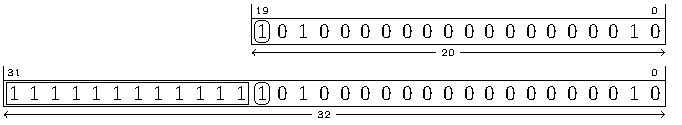
\includegraphics{figures/chapter02/SignExtendNegative.pdf}
\captionof{figure}{Sign-extending a negative integer from 20 bits to 32 bits.}
\label{Figure:SignExtendNegative}
\end{figure}

\autoref{Figure:SignExtendPositive} illustrates extending the sign bit of a
positive number to the left by replicating it.
A positive number will have its \acrshort{msb} set to 0.  Extending this
value to the left will set all the new bits to the left of it to 0 as well.

\begin{figure}[ht]
\centering
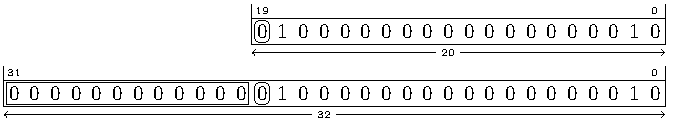
\includegraphics{figures/chapter02/SignExtendPositive.pdf}
\captionof{figure}{Sign-extending a positive integer from 20 bits to 32 bits.}
\label{Figure:SignExtendPositive}
\end{figure}


\label{ZeroExtension}
In a similar vein, any unsigned number also may have any quantity of
additional MSBs added to it provided that they are all zero.  This is
called {\em zero extension}.  For example,
the following all represent the same value:
\begin{verbatim}
                                   1111 <== 15
                                  01111 <== 15
          00000000000000000000000001111 <== 15
\end{verbatim}

\begin{tcolorbox}
Any {\em unsigned} number may be {\em zero extended} to any size.
\end{tcolorbox}

\ednote{Remove the sign-bit boxes from this figure?}%
\autoref{Figure:ZeroExtend} illustrates zero-extending a 20-bit number to the
left to form a 32-bit number.

\begin{figure}[ht]
\centering
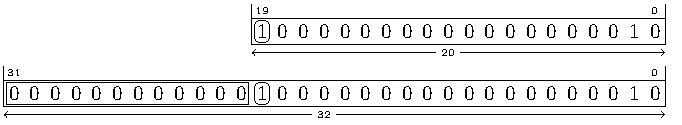
\includegraphics{figures/chapter02/ZeroExtend.pdf}
\captionof{figure}{Zero-extending an unsigned integer from 20 bits to 32 bits.}
\label{Figure:ZeroExtend}
\end{figure}

%Sign- and zero-extending binary numbers are common operations used to
%fit a byte or halfword into a fullword.

\section{Shifting}
\label{shifting}

We were all taught how to multiply and divide decimal numbers by ten
by moving (or {\em shifting}) the decimal point to the right or left
respectively.  Doing the same in any other base has the same effect
in that it will multiply or divide the number by its base.

\ednote{Include decimal values in the shift diagrams.}%
Multiplication and division are only two reasons for shifting.  There
can be other occasions where doing so is useful.

As implemented by a CPU, shifting applies to the value in a register
and the results stored back into a register of finite size.  Therefore
a shift result will always be truncated to fit into a register.

\ednote{Add some examples showing the rounding of positive and negative values.}%
Note that when dealing with numeric values, any truncation performed
during a right-shift will manifest itself as rounding toward zero.

\subsection{Logical Shifting}

Shifting {\em logically} to the left or right is a matter of re-aligning
the bits in a register and truncating the result.

\ednote{Redraw these with arrows tracking the shifted bits and the truncated values}%
To shift left two positions:

\begin{figure}[H]
  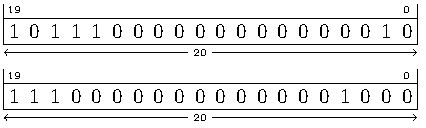
\includegraphics{figures/chapter02/ShiftLeftTwo.pdf}
  \label{Figure:ShiftLeftTwo}
\end{figure}

To shift right one position:

\begin{figure}[H]
  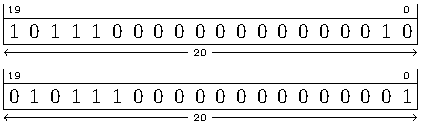
\includegraphics{figures/chapter02/ShiftRightOne.pdf}
  \label{Figure:ShiftRightOne}
\end{figure}

\begin{tcolorbox}
Note that the vacated bit positions are always filled with zero.
\end{tcolorbox}

\subsection{Arithmetic Shifting}

Some times it is desirable to retain the value of the sign bit when
shifting.  The RISC-V ISA provides an arithmetic right shift
instruction for this purpose (there is no arithmetic left shift for
this ISA.)

\begin{tcolorbox}
When shifting to the right {\em arithmetically}, vacated bit positions are
filled by replicating the value of the sign bit.
\end{tcolorbox}

An arithmetic right shift of a negative number by 4 bit positions:

\begin{figure}[H]
  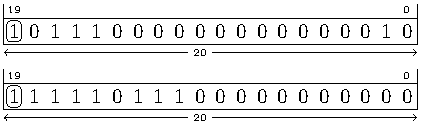
\includegraphics{figures/chapter02/ShiftNegativeNumberRightFour.pdf}
  \label{Figure:ShiftNegativeNumberRightFour}
\end{figure}

\section{Main Memory Storage}

As mentioned in \autoref{VolatileStorage}, the main memory in a RISC-V
system is byte-addressable.  For that reason we will visualize it by
displaying ranges of bytes displayed in hex and in \gls{ascii}.  As will
become obvious, the ASCII part makes it easier to find text messages.%
\footnote{Most of the memory dumps in this text are generated by \gls{rvddt}
and are shown on a per-byte basis without any attempt to reorder their
values. Some other applications used to dump memory do not dump the bytes
in address-order!  It is important to know how your software tools operate
when using them to dump the contents of memory and/or files.}

\subsection{Memory Dump}

\listingRef{examples/chapter02/rvddt_memdump.out} shows a {\em memory dump} from the rvddt
`d' command requesting a dump starting at address \hex{00002600}
for the default quantity (\hex{100}) of bytes.

\listing{examples/chapter02/rvddt_memdump.out}{{\tt rvddt} memory dump}

\begin{itemize}
\item [$\ell$ 1] The rvddt prompt showing the dump command.
\item [$\ell$ 2] From left to right. the dump is presented as the address
	of the first byte (\hex{00002600}) followed by a colon, the value
	of the byte at address \hex{00002600} expressed in hex, the next byte
	(at address \hex{00002601}) and so on for 16 bytes. There is a
	double-space
	between the 7th and 8th bytes to help provide a visual reference for
	the center to make it easy to locate bytes on the right end.  For
	example, the byte at address \hex{0000260c} is four bytes to the
	right of byte number eight (at the gap) and contains \hex{13}.
	To the right of the 16-bytes is an asterisk-enclosed set of 16 columns
	showing the ASCII characters that each byte represents.  If a byte
	has a value that corresponds to a printable character code, the character
	will be displayed.  For any illegal/un-displayable byte values, a dot
	is shown to make it easier to count the columns.
\item [$\ell$ 3-17] More of the same as seen on $\ell$ 2.  The address
	at the left can be seen to advance by $16_{10}$ (or $10_{16}$)
	for each line shown.
\end{itemize}

\subsection{Endianness}

The choice of which end of a multi-byte value is to be stored at the
lowest byte address is referred to as {\em endianness.}  For example,
if a CPU were to store a \gls{halfword} into memory, should the byte
containing the \acrfull{msb} (the {\em big} end) go first or does
the byte with the \acrfull{lsb} (the {\em little} end) go first?

On the one hand the choice is arbitrary.  On the other hand, it is
possible that the choice could impact the performance of the system.%
\footnote{See\cite{IEN137} for some history of the big/little-endian ``controversy.''}

IBM mainframe CPUs and the 68000 family store their bytes in big-endian
order.  While the Intel Pentium and most embedded processors use
little-endian order.
Some CPUs are even {\em bi-endian} in that they have instructions that
can change their order on the fly.

The RISC-V system uses the little-endian byte order.

\subsubsection{Big-Endian}
\label{BigEndian}
\index{big-endian}

Using the contents of \listingRef{rvddt_memdump.out}, a \gls{bigendian}
CPU would interpret the contents as follows:

\begin{itemize}
\item The 8-bit value read from address \colorbox{c_lightblue}{\hex{00002658}} would be \verb@0x@{\color{red}\verb@76@}.
\item The 8-bit value read from address \hex{00002659} would be \hex{61}.
\item The 8-bit value read from address \hex{0000265a} would be \hex{6c}.
\item The 8-bit value read from address \hex{0000265b} would be \hex{3d}.
\item The 16-bit value read from address \colorbox{c_lightblue}{\hex{00002658}} would be \verb@0x@{\color{red}\verb@76@}\verb@61@.
\item The 16-bit value read from address \hex{0000265a} would be \hex{6c3d}.
\item The 32-bit value read from address \colorbox{c_lightblue}{\hex{00002658}} would be \verb@0x@{\color{red}\verb@76@}\verb@616c3d@.
\end{itemize}

Notice that in a big-endian system, the {\em\gls{place-value}s} of the bits
comprising the \verb@0x@{\color{red}\verb@76@}
(located at memory address \colorbox{c_lightblue}{\hex{00002658}}) are
{\em different} depending on the number of bytes representing the value that is being read.

For example, when a 16-bit value is read from \colorbox{c_lightblue}{\hex{00002658}}
then the {\color{red}\verb@76@} represents
the binary place values: $2^{15}$ to $2^8$.
When a 32-bit value is read then the {\color{red}\verb@76@} represents
the binary place values: $2^{31}$ to $2^{24}$.
In other words the value read from the first memory location (with the
lowest address), of the plurality of addresses containing the complete
value being read, is always placed on the {\em left end}, into the
Most Significant Bits.  One might dare say that the {\color{red}\verb@76@}
is placed at the end with the {\em big} place values.

More examples:

\begin{itemize}
\item An 8-bit value read from address \colorbox{c_lightgreen}{\hex{00002624}} would be \verb@0x@{\color{red}\verb@23@}.
\item An 8-bit value read from address \hex{00002625} would be \hex{24}.
\item An 8-bit value read from address \hex{00002626} would be \hex{81}.
\item An 8-bit value read from address \hex{00002627} would be \hex{00}.
\item A 16-bit value read from address \colorbox{c_lightgreen}{\hex{00002624}} would be \verb@0x@{\color{red}\verb@23@}\verb@24@.
\item A 16-bit value read from address \hex{00002626} would be \hex{8100}.
\item A 32-bit value read from address \colorbox{c_lightgreen}{\hex{00002624}} would be \verb@0x@{\color{red}\verb@23@}\verb@248100@.
\end{itemize}

Again, notice that the byte from memory address \colorbox{c_lightgreen}{\hex{00002624}},
regardless of the {\em number} of bytes comprising the complete value being
fetched, will always appear on the left/{\em big} end of the final value.


\begin{tcolorbox}
On a big-endian system, the bytes in the dump are in the same order as
they would be used by the CPU if it were to read them as a multi-byte
value.
\end{tcolorbox}

\subsubsection{Little-Endian}
\label{LittleEndian}
\index{little-endian}

Using the contents of \listingRef{rvddt_memdump.out}, a \gls{littleendian}
CPU would interpret the contents as follows:

\begin{itemize}
\item An 8-bit value read from address \colorbox{c_lightblue}{\hex{00002658}} would be \verb@0x@{\color{red}\verb@76@}.
\item An 8-bit value read from address \hex{00002659} would be \hex{61}.
\item An 8-bit value read from address \hex{0000265a} would be \hex{6c}.
\item An 8-bit value read from address \hex{0000265b} would be \hex{3d}.
\item A 16-bit value read from address \colorbox{c_lightblue}{\hex{00002658}} would be \verb@0x61@{\color{red}\verb@76@}.
\item A 16-bit value read from address \hex{0000265a} would be \hex{3d6c}.
\item A 32-bit value read from address \colorbox{c_lightblue}{\hex{00002658}} would be \verb@0x3d6c61@{\color{red}\verb@76@}.
\end{itemize}

Notice that in a little-endian system, the {\em\gls{place-value}s} of the bits
comprising the \verb@0x@{\color{red}\verb@76@}
(located at memory address \colorbox{c_lightblue}{\hex{00002658}})
are the {\em same} regardless of the the number of bytes representing the value that is being read.

Unlike the behavior of a big-endian machine, when little-endian machine
reads a 16-bit value from \colorbox{c_lightblue}{\hex{00002658}} the
{\color{red}\verb@76@} represents the binary place values from $2^{7}$ to $2^0$.
When a 32-bit value is read then the {\color{red}\verb@76@} (still) represents
the binary place values from $2^{7}$ to $2^{0}$.
In other words the value read from the first memory location (with the
lowest address), of the plurality of addresses containing the complete
value being read, is always placed on the {\em right end}, into the
Least Significant Bits.  One might say that the {\color{red}\verb@76@}
is placed at the end with the {\em little} place values.

Also notice that it is the {\em bytes} are what are ``reversed'' in a little-endian
system ({\em not} the hex digits.)

More examples:

\begin{itemize}
\item The 8-bit value read from address \colorbox{c_lightgreen}{\hex{00002624}} would be \verb@0x@{\color{red}\verb@23@}.
\item The 8-bit value read from address \hex{00002625} would be \hex{24}.
\item The 8-bit value read from address \hex{00002626} would be \hex{81}.
\item The 8-bit value read from address \hex{00002627} would be \hex{00}.
\item The 16-bit value read from address \colorbox{c_lightgreen}{\hex{00002624}} would be \verb@0x24@{\color{red}\verb@23@}.
\item The 16-bit value read from address \hex{00002626} would be \hex{0081}.
\item The 32-bit value read from address \colorbox{c_lightgreen}{\hex{00002624}} would be \verb@0x008124@{\color{red}\verb@23@}.
\end{itemize}

As above, notice that the byte from memory address \colorbox{c_lightgreen}{\hex{00002624}},
regardless of the {\em number} of bytes comprising the complete value being
fetched, will always appear on the right/{\em little} end of the final value.

\begin{tcolorbox}
On a little-endian system, the bytes in the dump are in reverse order as
they would be used by the CPU if it were to read them as a multi-byte value.
\end{tcolorbox}

In the RISC-V ISA it is noted that
\begin{quote}
A minor point is that we have also found
little-endian memory systems to be more natural for hardware
designers. However, certain application areas, such as IP networking, operate
on big-endian data structures, and so we leave open the possibility of
non-standard big-endian or bi-endian systems.''\cite[p.~6]{rvismv1v22:2017}
\end{quote}

\subsection{Arrays and Character Strings}

While Endianness defines how single values are stored in memory,
the {\em array} defines how multiple values are stored.

An array is a data structure comprised of an ordered set of elements.
This text will limit its definition of array to a plurality of
elements that are all of the same type.  Where type
refers to the size (number of bytes) and representation (signed,
unsigned,\ldots) of each element.

In an array, the elements are stored adjacent to one another such that the
address $e$ of any element $x[n]$ is:

\begin{equation}
e = a + n * s
\end{equation}

Where $x$ is the name of the array, $n$ is the element number of interest,
$e$ is the address of interest, $a$ is the address of the first element in
the array and $s$ is the size (in bytes) of each element.

Given an array $x$ containing $m$ elements, $x[0]$ is the first element of
the array and $x[m-1]$ is the last element of the array.%
\footnote{Some computing languages (C, C++, Java, C\#, Python, Perl,\ldots)
define an array such that the first element is indexed as $x[0]$.
While others (FORTRAN, MATLAB) define the first element of an
array to be $x[1]$.}

Using this definition, and the memory dump shown in
\listingRef{rvddt_memdump.out}, and the knowledge that
we are using a little-endian machine and given that
$a = $ \hex{00002656} and $s = 2$, the values of the first 8 elements
of array $x$ are:

\begin{itemize}
\item $x[0]$ is \hex{0000} and is stored at \hex{00002656}.
\item $x[1]$ is \hex{6176} and is stored at \hex{00002658}.
\item $x[2]$ is \hex{3d6c} and is stored at \hex{0000265a}.
\item $x[3]$ is \hex{0000} and is stored at \hex{0000265c}.
\item $x[4]$ is \hex{0000} and is stored at \hex{00002660}.
\item $x[5]$ is \hex{0000} and is stored at \hex{00002662}.
\item $x[6]$ is \hex{8480} and is stored at \hex{00002664}.
\item $x[7]$ is \hex{412e} and is stored at \hex{00002666}.
\end{itemize}

\begin{tcolorbox}
In general, there is no fixed rule nor notion as to how many
elements an array has.  It is up to the programmer to ensure that
the starting address and the number of elements in any given array
(its size) are used properly so that data bytes outside an array
are not accidentally used as elements.
\end{tcolorbox}

There is, however, a common convention used for an array of
characters that is used to hold a text message
(called a {\em character string} or just {\em string}).

When an array is used to hold a string the element past the last
character in the string is set to zero.  This is because 1) zero
is not a valid printable ASCII character and 2) it simplifies
software in that knowing no more than the starting address of a
string is all that is needed to processes it.  Without this zero
{\em sentinel} value (called a {\em null} terminator), some knowledge
of the number of characters in the string would have to otherwise
be conveyed to any code needing to consume or process the string.

In \listingRef{rvddt_memdump.out}, the 5-byte long array starting
at address \hex{00002658} contains a string whose value can be
expressed as either: % \verb@76 61 6c 3d 00@ or \verb@"val="@.

\verb@76 61 6c 3d 00@

or

\verb@"val="@

%\begin{itemize}
%\item \verb@76 61 6c 3d 00@
%\item \verb@"val="@
%\end{itemize}

\index{ASCII}
\index{ASCIIZ}
When the double-quoted text form is used, the GNU assembler used in
this text differentiates between {\em ascii} and {\em asciiz} strings
such that an {\em ascii} string is {\bf not} null terminated and an
{\em asciiz} string {\bf is} null terminated.

The value of providing a method to create a string that is not
null terminated is that a program may define a large string by
concatenating a number of {\em ascii} strings together and following the
last with a byte of zero to null-terminate it.

It is a common mistake to create a string with a missing
null terminator.  The result of printing such a string is that
the string will be printed as well as whatever random data bytes in
memory follow it until a byte whose value is zero is encountered
by chance.

\subsection{Context is Important!}

Data values can be interpreted differently depending on the context in
which they are used.  Assuming what a set of bytes is used for based on
their contents can be very misleading!  For example, there is a 0x76 at
address 0x00002658.  This is a `v' is you use it as an ASCII
(see~\autoref{chapter:ascii}) character, a $118_{10}$ if it is an integer
value and TRUE if it is a conditional.

\subsection{Alignment}

\ednote{Include the obligatory diagram showing the overlapping data types
when they are all aligned.}%
With respect to memory and storage, {\em \gls{alignment}} refers to the
{\em location} of a data element when the address that it is stored is
a precise multiple of a power-of-2.

The primary alignments of concern are typically 2 (a halfword),
4 (a fullword), 8 (a double word) and 16 (a quad-word) bytes.

For example, any data element that is aligned to 2-byte boundary
must have an (hex) address that ends in any of: 0, 2, 4, 6, 8, A,
C or E.
Any 4-byte aligned element must be located at an address ending
in 0, 4, 8 or C.  An 8-byte aligned element at an address ending
with 0 or 8, and 16-byte aligned elements must be located at
addresses ending in zero.

Such alignments are important when exchanging data between the CPU
and memory because the hardware implementations are optimized to
transfer aligned data.  Therefore, aligning data used by any program
will reap the benefit of running faster.%
\footnote{Alignment of data, while important for efficient performance,
is not mandatory for RISC-V systems.\cite[p.~19]{rvismv1v22:2017}}

An element of data is considered to be {\em aligned to its natural size}
when its address is an exact multiple of the number of bytes used to
represent the data.  Note that the ISA we are concerned with {\em only}
operates on elements that have sizes that are powers of two.

For example, a 32-bit integer consumes one full word.  If the four bytes
are stored in main memory at an address than is a multiple of 4 then
the integer is considered to naturally aligned.

The same would apply to 16-bit, 64-bit, 128-bit and other such values
as they fit into 2, 8 and 16 byte elements respectively.

Some CPUs can deliver four (or more) bytes at the same time while others
might only be capable of delivering one or two bytes at a time.  Such
differences in hardware typically impact the cost and performance of a
system.%
\footnote{The design and implementation
choices that determine how any given system operates are part of what is
called a system's {\em organization} and is beyond the scope of this text.
See~\cite{codriscv:2017} for more information on computer organization.}

\subsection{Instruction Alignment}

The RISC-V ISA requires that all instructions be aligned to their
natural boundaries.

Every possible instruction that an RV32I CPU can execute contains
exactly 32 bits.  Therefore they are always stored on a full word
boundary.  Any {\em unaligned} instruction is {\em illegal}.%
\footnote{This rule is relaxed by the C extension to allow an
instruction to start at any even address.\cite[p.~5]{rvismv1v22:2017}}

An attempt to fetch an instruction from an unaligned address
will result in an error referred to as an alignment {\em \gls{exception}}.
This and other exceptions cause the CPU to stop executing the
current instruction and start executing a different set of instructions
that are prepared to handle the problem.  Often an exception is
handled by completely stopping the program in a way that is commonly
referred to as a system or application {\em crash}.